\section{A brief history of character graphics}
\label{sec:terminals}
\epigraph{Let's take it back to '79!}{Wu-Tang Clan \xelatexemoji{f0000}, ``Triumph''}
The earliest terminals making use of glyphs\footnote{Konrad Zuse's Z3, generally
 considered the first programmable digital computer, communicated with its
operator through a matrix of blinkenlights and a not unsteampunkish keyboard that resembled the
Burroughs typewriters of its era\cite{zuse}.} printed them to paper, and are of
interest to us only so far as our modern term ``tty'' is rather dubiously
derived from ``TeleTYpewriter'', as these cantankerous contraptions were
known\footnote{Though we do hear of their Snoopy calendars in the songs of
legend\cite{quiche}.} (people had less experience abbreviating in those days).

These devices most typically printed 72 characters per line (CPL), a limit that
has persisted in strange places\cite{pandoc} through the modern era. Another constant
you'll see from time to time is 132 CPL, derived from line printers such as the
IBM 1403, the DEC LP11, and the Centronics 101\cite{ibm1403}. Most common,
however, is the 80 column line originating in 1928's 7¾x3¼x0.007in IBM
Computer Card (as designed by Clair D.\ Lake, borrowing from the 1890 U.\ S.\
Census cards of Herman Hollerith\ldots themselves inspired by Joseph
Jacquard's automation in 1804 of punched card loom control technology pioneered
by Basile Bouchon in 1725\cite{cards}). To this day, so long as your wacky
output device can do 80 columns, eh, that's good enough. In all these cases,
the limit arises from the number of characters that could be printed, using the
technology of the time, on their feeder paper (8.5in and 14in in the case of
printers).

On, then, to the ``Glass TTYs'' (ugh) and Visual Display Units of the 1970s.
Pictured in Figure~\ref{fig:terminals} are the Computer Terminal Corporation
Datapoint 3300, the Lear Sigler, Inc.\ ADM-3A, the Hazeltine 1500, and the
Soroc IQ-120. Lacking microcontrollers, and generally implementing no
independent control sequences, such devices are today often known as ``dumb
terminals'' (this term was originally a registered trademark of Lear Sigler,
see Figure~\ref{fig:adm3}). Already the 80x24 ``standard'' (it is not a standard) was emerging
(the DEC contemporaries listed were already pretty ``smart'', using proprietary
control codes):

\begin{table}[h]
\begin{center}
  \begin{tabular}{ |c|c|c| }
    \hline
    IBM 2260 Model 1 & 1965 & 40x6 \\
    \hline
    Datapoint 3300 & 1969 & 72x25 \\
    \hline
    DEC VT05 & 1970 & 72x24 \\
    \hline
    IBM 3277 Model 2 & 1971 & 80x24 \\
    \hline
    Textronix 4010 & 1972 & 74x35 \\
    \hline
    DECscope VT52 & 1974 & 80x24 \\
    \hline
    LSI ADM-3A & 1976 & 80x12, 80x24 \\
    \hline
    Hazeltine 1500 & 1977 & 80x24 \\
    \hline
    Sororc IQ-120 & 1977 & 80x24 \\
    \hline
  \end{tabular}
\caption{Some historical terminals and their resolutions.}
\end{center}
\end{table}

Why 80x24 (or 80x25, as you'll also see)\cite{infoworld80}? The 80 almost certainly arises from
the desire to display an entire punched card (this \textit{is} a standard---see
ANSI X3.21-1967/FIPS PUB 13, ``Rectangular Holes in Twelve-Row Punched
Cards'')\cite{sonicdelay}. The origin of 24 is less clear. 24 is highly
composite (it has more divisors than any smaller number), and it is the largest
integer divisible by all natural numbers not larger than its square root. There
are of course 24 hours in a day. 24 divides the scanline counts of both NTSC
and PAL at 480 and 576, respectively. 24 rows of 80 columns at a byte per
column utilize 93.75\% of a 2KiB memory, leaving exactly 128 bytes left over,
and everyone loves a good power of 2.

The Aaronites, Levite descendents of Moses's brother Aaron, the first
\texthebrew{כהן גדול}
(High Priest),
form the priestly \texthebrew{כֹּהֲנִים}; they were divided into 24 courses. The Buddha's Dharma Chakra (Wheel of Dhamma)
in its Ashoka form sends forth 24 spokes. But perhaps I grow esoteric, even
speculative\ldots in truth, 80x24 almost certainly owes its questionable
existence to IBM's punched cards, IBM 2260 and 3270 wanting compatibility with
IBM printers, the upstart DEC wanting compatibility with IBM software for their
VT52 and legendary VT100, and the VT100 subsequently becoming a \textit{de facto} standard for
four decades.

\begin{figure}
  \centering 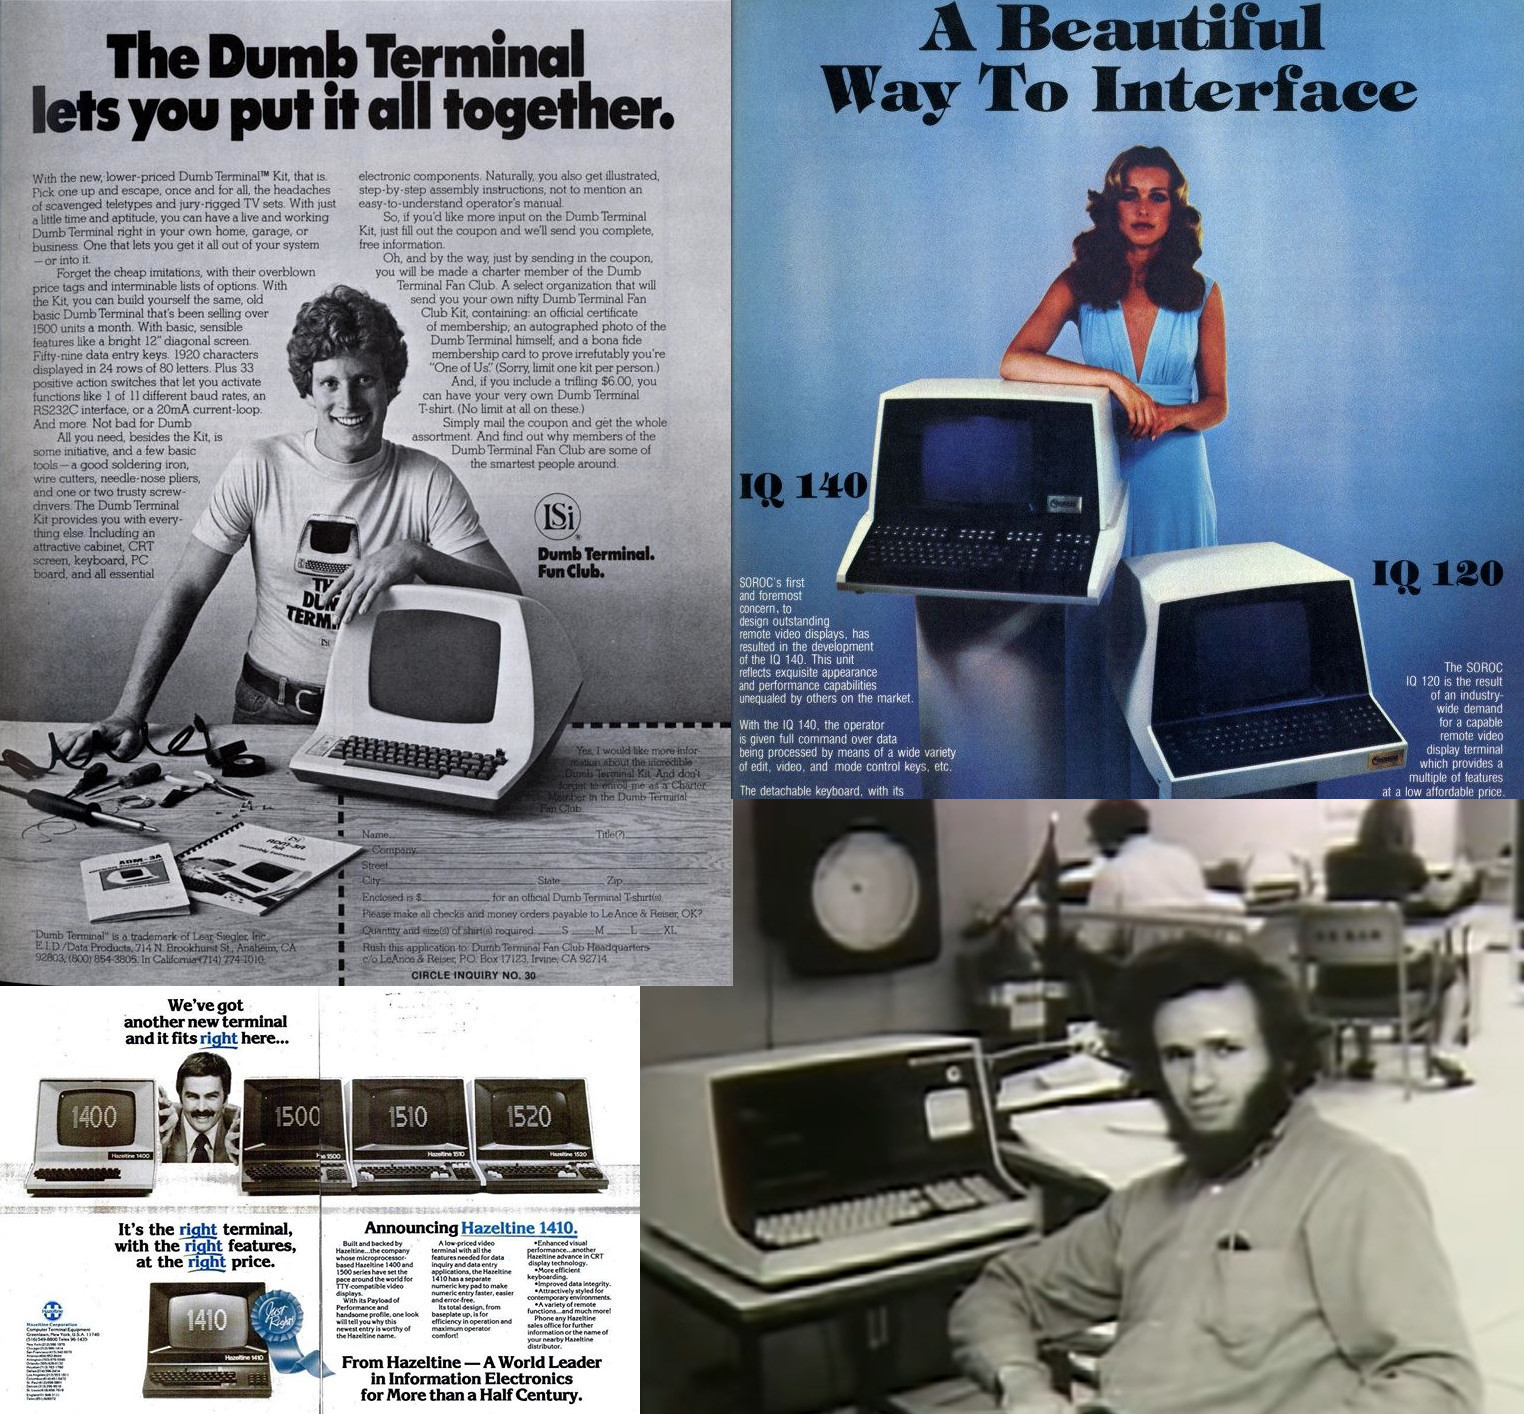
\includegraphics[width=.9\linewidth]{media/dumbterminals.jpg}
\caption[Dumb terminals of the 1970s.]{Clockwise starting from upper left: a dork and his LSI ADM (``American
  Dream Machine'', supposedly). That poor woman with the Sororc IQs looks stoned out
  of her gourd. Grizzly Adams rocks a Datapoint 3300, but really his mind is on
  seeing Skynyrd shred it this weekend. Finally, we have Frank the Cocaine
  Ranger and his Electric Hazeltine 1500 Band. \textit{Gott im Himmel}, the 70s were \textit{unseemly}.}
\label{fig:terminals}
\end{figure}

\begin{figure}
  \begin{minipage}{0.5\textwidth}
  \centering
    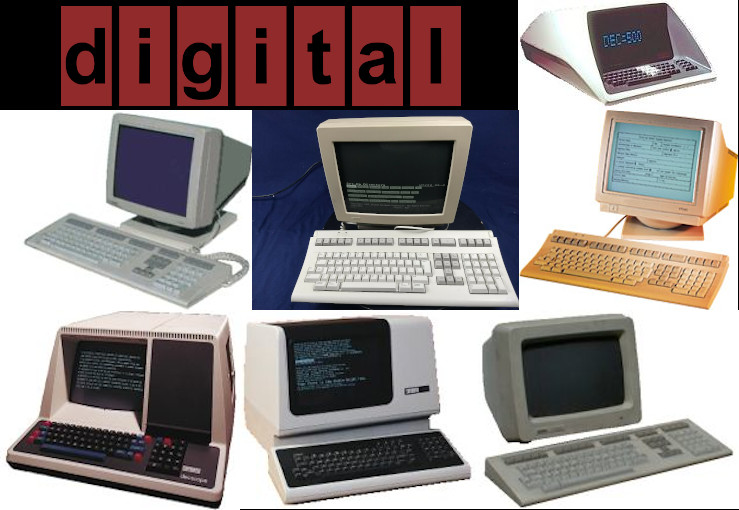
\includegraphics[width=.5\linewidth]{media/digital-terms.jpeg}
    \caption{Digital Equipment Corporation terminals of the 1970s and 1980s.}
  \end{minipage}\hfill
  \begin{minipage}{0.4\textwidth}
  \centering
    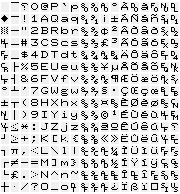
\includegraphics[width=.45\linewidth]{media/vt220-charset.png}
    \caption[VT220 glyph dump.]{The VT220's glyphs from a ROM dump. VT100 implemented most of the
      first seven columns. Note the existence of box-drawing characters\cite{crttypography}.}
  \end{minipage}\hfill
\end{figure}

\begin{figure}
  \centering
  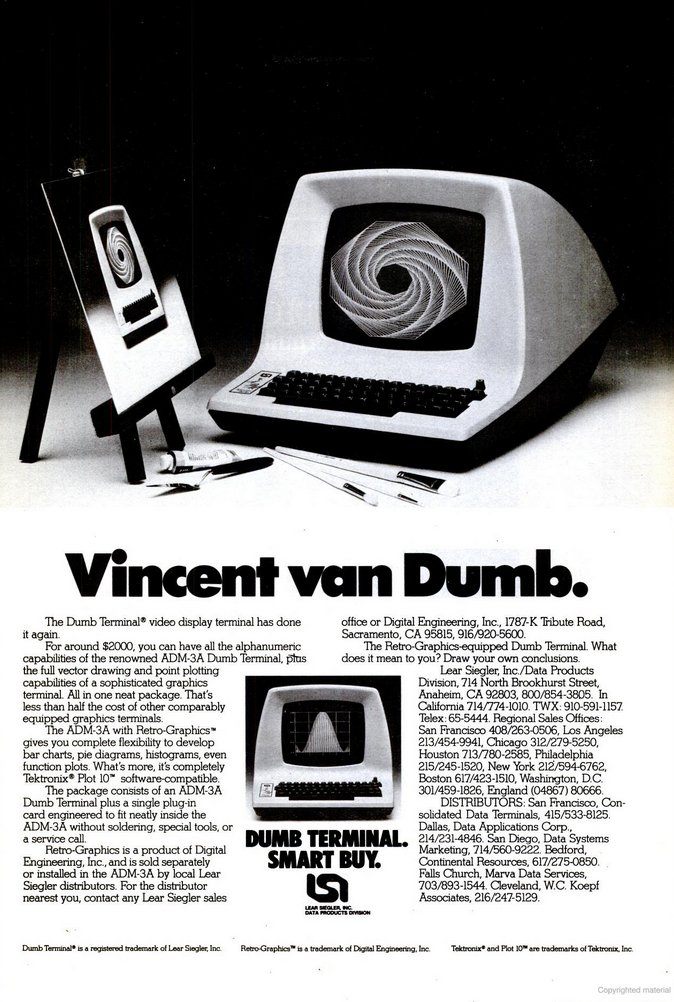
\includegraphics[width=.8\linewidth]{media/adm3.jpeg}
  \caption[]{A strange time.}
  \label{fig:adm3}
\end{figure}

\subsection{The DEC VTxxx terminals and ANSI X3.64-1979}

Introduced in August 1978, the VT100 ushered in a new era of smart terminals
using commodity (Intel) microprocessors, implementing portions of the upcoming
ANSI X3.64 standard (itself based on 1976's first edition of ECMA-48) along
with DEC extensions\footnote{The VT100 \textit{did not} implement all of X3.64,
nor was X3.64 derived from the VT100. The VT100 didn't do color, nor did it
insert or delete lines. It furthermore implemented several features outside
the scope of ECMA-48's first edition.} This series would go on to sell over
six million units, and it was a rare vendor that didn't include some degree
of DEC VT compatibility. Each major iteration of the series was designed to
encompass all functionality of prior iterations, beginning with the VT100's
faithful emulation of the earlier era's VT52\cite{vt52}. The VT102 cut down on the cost
and size of the VT100, and included the 132-CPL mode by default; they were
otherwise essentially the same device\cite{vt100}.

Terminals had quite a heyday through the 1970s and 1980s, but as the price of
Wintel machines fell below \$1,000, their value proposition rapidly eroded.
They lived on, especially in niche minicomputer and mainframe installations,
but as of 2020 it's difficult to find a new terminal. Digital sold their
terminal business to SunRiver Data Systems (now Boundless Technologies) in
1995; the \url{boundlessterminals.com} site is not offered over HTTPS, and
reads ``Now it is time for the last text terminals to give way to newer
technologies\cite{boundless}.'' Press F to pay respects.

The original \texttt{xterm} (released in X10R3) was written as an emulator of
the VAXStation 100 (VS100), and slowly acquired scattered features from the
VT100, ANSI, and other sources\cite{xtermfaq}. Thomas E.\ Dickey (the current
maintainer of \Gls{ncurses} and xterm) began working on XTerm in the mid-90s,
and by 1996 had added the \texttt{decTerminalID} resource following the
addition of much VT220 compatibility. \texttt{xterm} can be built with support
for Sixel, ReGIS, Unicode, and an extraordinary number of archaic and/or
baroque mechanics with which I'm not personally familiar. Further information
is available in Mr.\ Dickey's
\href{https://invisible-island.net/xterm/xterm.faq.html}{XTerm FAQ}, which
makes for excellent reading\footnote{Mr.\ Dickey's XTerm and NCURSES FAQs are,
in my opinion, two of the finest pieces of technical documentation in
existence. It is my hope that this manuscript approaches their level.}.

I will not attempt to list the hundreds (probably thousands) of terminal
emulators that are available. Most claim some manner of ``ANSI'' or ``vt100''
(not the same thing!) compliance; take these claims with a large grain of salt.
It's worth knowing about:

\begin{denseitemize}
\item{\texttt{rxvt}, ``Rob's \texttt{xvt}''. An enhancement of \texttt{xvt} touted
    as a slimmed-down, simplified alternative to \texttt{xterm}. Implemented pixel-addressable
    graphics (in a scheme incompatible with Sixel). Like \texttt{xterm}, it uses
    X resources for configuration. Various forks add various essential technologies
    introduced since 2000.}
\item{Konsole, the official terminal of KDE. Having never used KDE substantially,
   I've never made much use of Konsole. I recall it having URL recognition
   when most terminal emulators didn't.}
\item{VTE terminals, a family of terminals built around GNOME's VTE library, built
  atop GTK3. GNOME and Xfce's terminals both wrap VTE, as do dozens of others.
  \texttt{xfce4-terminal} plays the role of our VTE terminal in benchmarks, because
  I run XFCE (atop Compiz).}
\item{\texttt{alacritty}, written in Rust by Joe Wilm. One of the new class of
    emulators written directly against OpenGL.}
\item{\texttt{kitty}, another OpenGL program, this one in C++/Python by Kovid Goyal.}
\item{Terminology is the emulator of Enlightenment since E17, the long (twelve
    years!) awaited successor to E16. It seemed somewhat broken every time I
    tried it, and by 2014 I didn't want to spend time fixing terminal emulators.
    It does look really pretty on its website\cite{terminology}.}
\item{Terminator was written in Java, which\textellipsis life finds a way I guess.}
\end{denseitemize}

I haven't benchmarked \texttt{rxvt} because I didn't care to figure out which of
its ten thousand forks is the one you're supposed to use. Likewise, I didn't
benchmark Terminator because I would prefer setting myself on fire
to running a Java terminal emulator.

The best single source of terminal emulator (and terminal) information is
probably the ``Terminal Type Descriptions'' file distributed with NCURSES\cite{termdescript}.

\subsection{The Curses API}
Several APIs for TUIs and character (semi)graphics have emerged over the fifty
years of video terminals' existence. Of them, by far the most venerable,
portable, and proven is Curses, which has (for over twenty years) actually
been codified in the Single UNIX Specification. Notcurses is an obvious
intellectual descendant of Curses, and indeed ought be easy to pick up by any
experienced Curses programmer.

As mentioned in Chapter~\ref{sec:terminfo}, Ken Arnold released the first BSD
Curses library shortly after extracting \texttt{vi}'s terminal abstraction routines
as libtermcap, and that first Curses made use of termcap\cite{cursesexplained}.
Similarly to termcap, Curses had its origins in Joy's \texttt{vi} code; unlike
termcap, Curses required significant reworking to be presented as a sensible
API. Meanwhile, over in AT\&T land, Mary Ann Horton (previously maintainer of
BSD's \texttt{vi} and \texttt{termcap}) arrived and implemented a new Curses,
this one making use of her terminfo. The two diverged over the years (with PDCurses
aka Public Domain Curses reimplementing AT\&T to work around licensing issues),
until X/Open codified an official vendor-neutral Curses, publishing it in
1996's Issue 4, version 2 (this specification derived primarily from SVR4 Curses).

Zeyd Ben-Halim adapted ncurses from the pcurses project of Pavel Curtis. Dickey
reports the 1.8.1 version released 1993-11-05 (and included with Slackware 2.0.1)
as the ``first widely-used version''. Numerous people (including the notorious
Eric S. Raymond and Ulrich Drepper) contributed significant code, but most NCURSES
development in recent years has been the work of Thomas Dickey.

The Curses API is best reviewed by reading the comprehensive man pages installed
with NCURSES. A few lines follow, summarizing major differences between Curses and Notcurses:

\begin{denseitemize}
\item{Curses has no built-in concept of a z-axis without use of its Panels
    extension, and its \texttt{stdscr} (analogous to the standard plane of
    Notcurses) is not considered part of the Panels stack. Curses does, however,
    allow windows to share memory, a capability Notcurses does not yet offer.}
\item{Panels can be ``hidden'', i.e.\ removed from the z-axis entirely. This cannot
    be done in Notcurses (but planes can be hidden underneath an opaque plane,
    or moved outside the visible area).}
\item{NCURSES defines its color API in terms of ``color pairs''. It is true that some
    terminals require both colors to be changed at the same time, but Notcurses
    hides this fact from the programmer, and instead allows foregrounds and backgrounds
    to be specified wholly independently.}
\item{Curses does not include the Panel, Menu, or Form extensions distributed
    with NCURSES. With that said, their presence in NCURSES effectively means
    they're in Curses. Notcurses is built around a Panel-like concept, and
    includes menus in its base, but lacks the rich Forms capabilities of NCURSES.}
\item{NCURSES supports only up to 256 colors at a time, as components of up to
    32,767 color pairs. There are no such limits in Notcurses (assuming terminal support).}
\item{NCURSES considers it an error to move a window or cursor off the screen. This
    is not an error in Notcurses.}
\end{denseitemize}
